\documentclass{beamer}

\usepackage[T1,T2A]{fontenc}
\usepackage[utf8]{inputenc}
\usepackage[russian, english]{babel}

\usepackage{amsmath, amsfonts, amsthm, amscd}
%\usepackage{graphics}
\usepackage{graphicx}
\usepackage[matrix,arrow,curve]{xy}
%\usepackage{multicol}

%----------------------------------------------------

\newtheorem{problemR}{Проблема}
\newtheorem{aim}{Цель}


\newtheorem{construction}{Construction}
\newtheorem{problems}{Problems}
\newtheorem{conjecture}{Conjecture}
\newtheorem{question}{Question}

\mode<presentation>
\usetheme{Madrid}


\begin{document}
\date{25 июня, 2022}


\begin{frame}
\begin{center}


{\large \scshape

\bigskip

\bigskip

Сервис поиска соседних объектов

\bigskip
\bigskip
\bigskip
\bigskip
\bigskip
\bigskip
}



Выполнил: Амеличев Константин, ПМИ 195\\
\bigskip
Научный руководитель: Тощев Андрей Александрович, Tinkoff.ru


\end{center}
\end{frame}

% \begin{frame}

% \frametitle{Проблема}

% В продуктовой разработке регулярно встречается вспомогательная поисковая задача с различными конфигурациями. Нужно максимально универсальное решение для общего подхода.

% \end{frame}


\begin{frame}

\frametitle{Цель работы}

Создание <<универсального>> поискового сервиса SimSearch (от англ. \textit{similarity search}).

\bigskip

Поисковый объект --- что угодно, что можно векторизовать с сохранением свойств.

\begin{center}
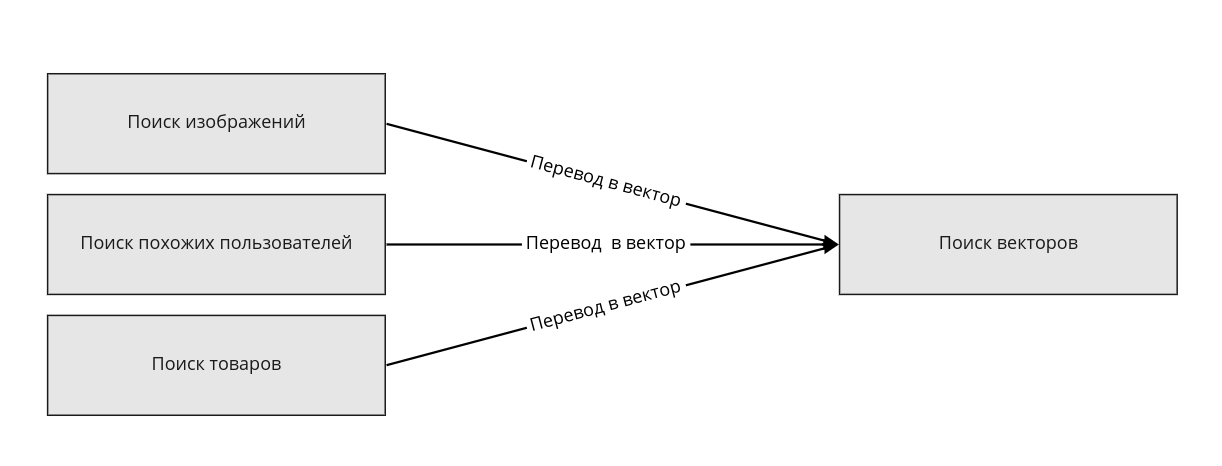
\includegraphics[width=0.8\linewidth]{search_problem_approach.png}
\end{center}


\end{frame}

\begin{frame}

\frametitle{Требования к поисковому сервису}

\begin{itemize}
\item Гибкость при решении поисковой задачи 
\item Поддержка различных баз: как статических, так и динамически меняющихся
\item Быстрые ответы на запросы, даже при больших базах
\item Возможность масштабировать сервис
\end{itemize}

\end{frame}

\begin{frame}
\frametitle{SimSearch: актуальность и значимость}

Подобного сервиса в открытом доступе нет, только продукты, заточенные под конкретную поисковую задачу

\hfill

Преимущества SimSearch:

\begin{itemize}
\item Гибкость, которой нет у специализированных сервисов
\item Универсальность: в предлагаемую модель обобщается множество поисковых задач
\item Продвинутые применения: Multimodal space (поиск картинок по текстовому описанию)
\end{itemize}

\end{frame}

\begin{frame}

\frametitle{Поставленные задачи}

\begin{itemize}
\item Изучение задачи поиска ближайших векторов (ANN: \textit{approximate nearest neighbors})
\item Проектирование SimSearch
\item Разработка и тестирование SimSearch
\item Разработка поиска похожих изображений на основе SimSearch
\end{itemize}

\end{frame}

\begin{frame}

\frametitle{Задача ANN: изученные подходы}
\begin{center}

\begin{figure}
\begin{minipage}{4cm}
\centering
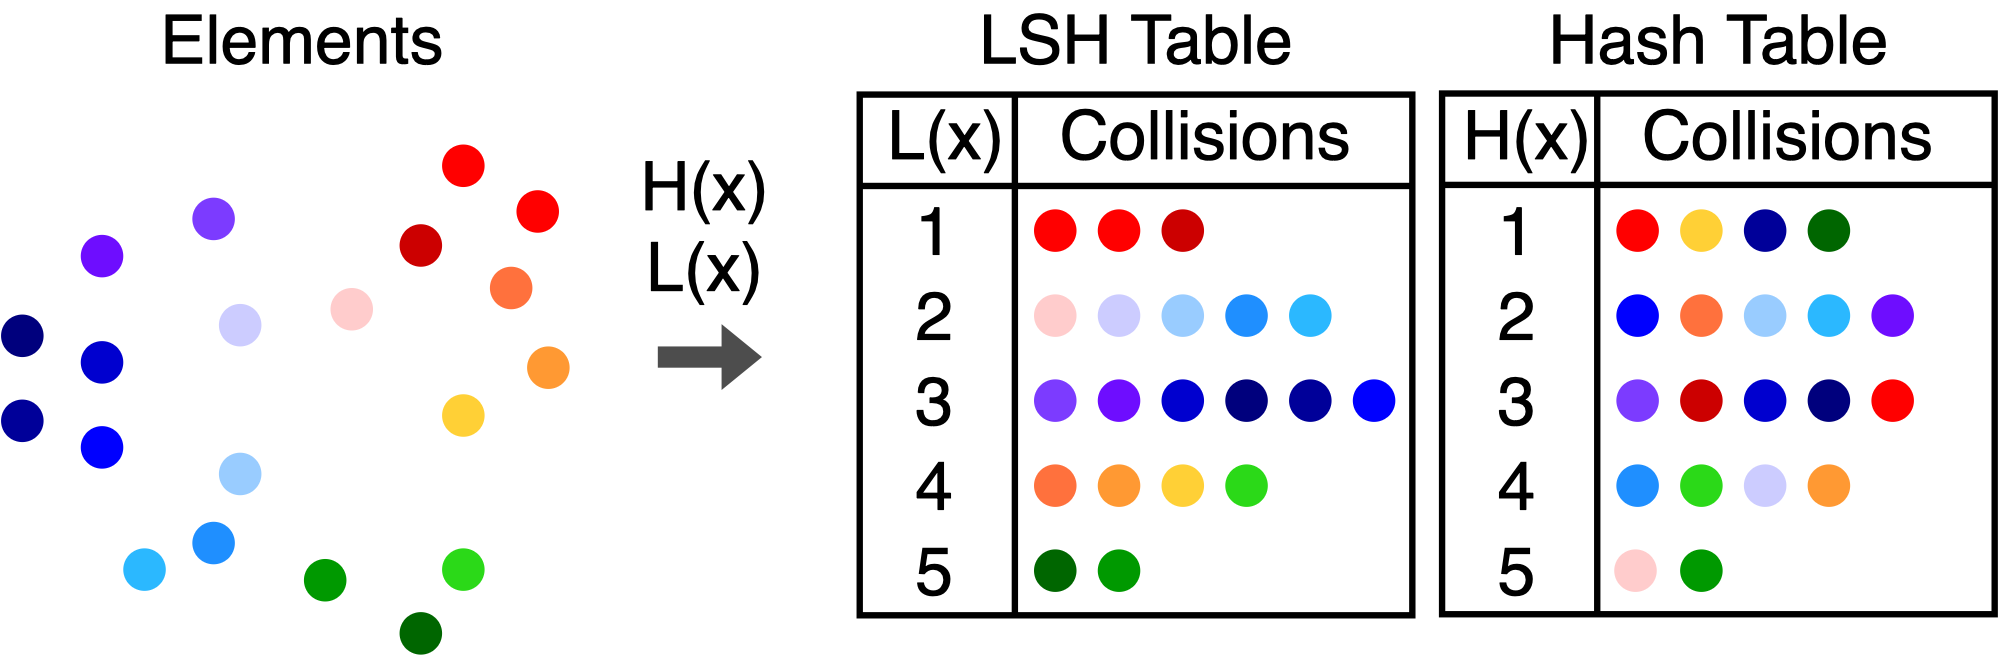
\includegraphics[width=3cm]{lsh_hashtable.png}

LSH
\end{minipage}
\begin{minipage}{4cm}
\centering
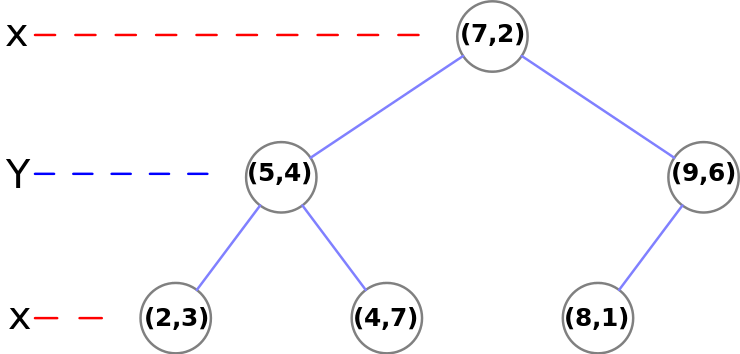
\includegraphics[width=3cm]{kdtree-tree.png}
KD-tree
\end{minipage}
\end{figure}
\begin{figure}
\begin{minipage}{4cm}
\centering

\includegraphics[width=3cm]{voronoi.png}
Quantization
\end{minipage}
\begin{minipage}{4cm}
\centering
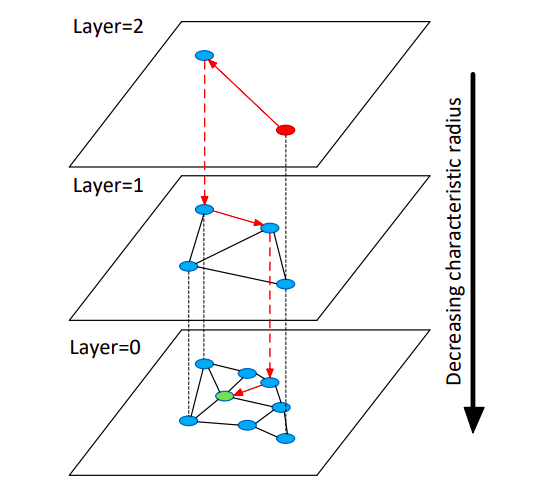
\includegraphics[width=3cm]{hnsw_graph.png}
HNSW
\end{minipage}
\end{figure}

\textbf{Вывод из исследования:} приоритетные подходы~--- LSH и HNSW.

\end{center}

\end{frame}

\begin{frame}

\frametitle{Задача ANN: Выбор библиотеки для LSH}

Выбор из open-source библиотек на C++:
\begin{itemize}
\item LSHKit
\item MyLSHBox
\item slash
\end{itemize}

\textbf{Выбор}: LSHKit для алгоритма LSH --- больше всего поддерживаемых расстояний и функций LSH, есть multi-probe lsh, lsh forest.

\end{frame}

\begin{frame}

\frametitle{Задача ANN: Выбор библиотеки для HNSW}

\begin{figure}
\centering
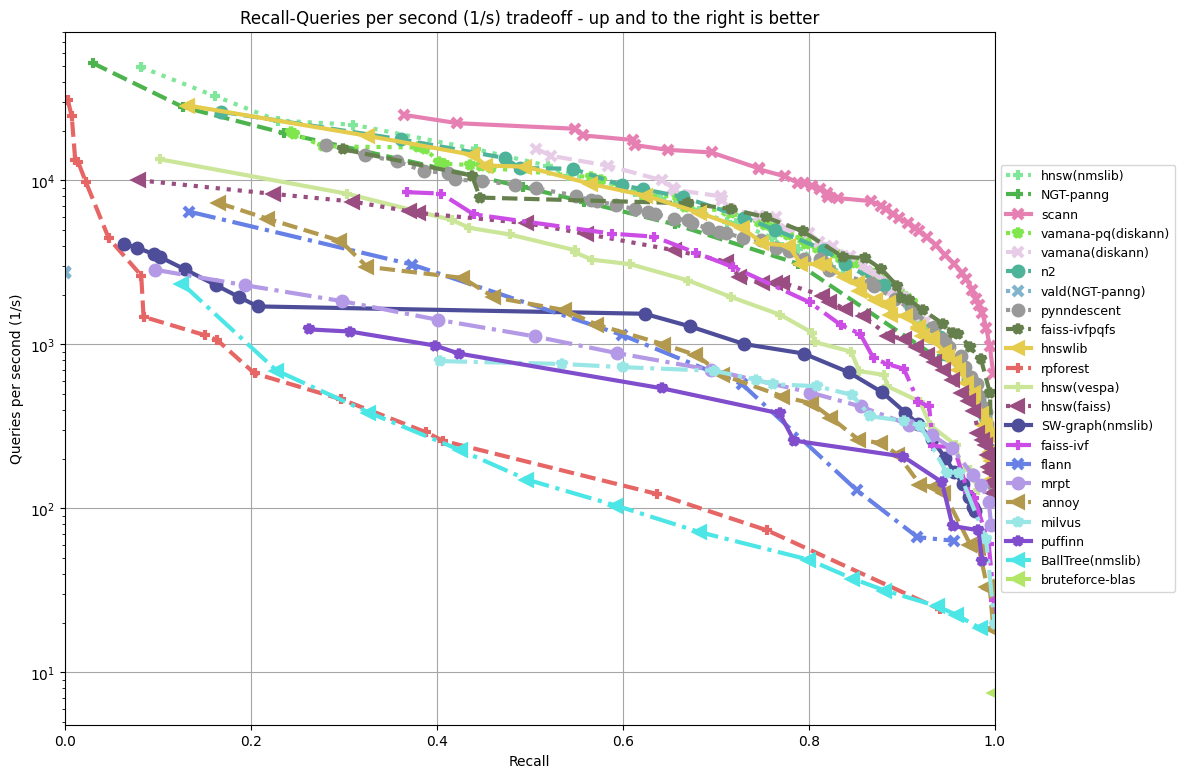
\includegraphics[width=8cm]{glove-100-angular_10_angular.png}

Тестирование на данных glove-100-angular (k = 10) [\href{ann-benchmark.com}{\color{blue}1}]
\end{figure}

\textbf{Выбор}: FaiSS для алгоритма HNSW --- хорошая скорость, содержит также другие алгоритмы (например, на основе квантизации).

\footnotetext[1]{ann-benchmark.com}

\end{frame}

\begin{frame}
\frametitle{SimSearch: проектирование}

\begin{center}
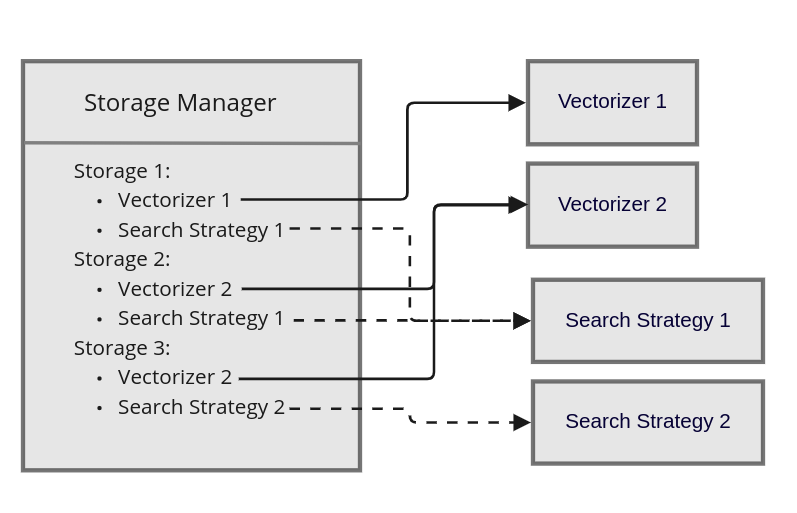
\includegraphics[width=0.7\linewidth]{miro_3.png}
\end{center}

Выделяем векторизацию и стратегию поиска в разные модули. Благодаря общему интерфейсу модули можно комбинировать и эффективно переиспользовать!

\end{frame}
\begin{frame}
\frametitle{SimSearch: архитектура}

\begin{center}
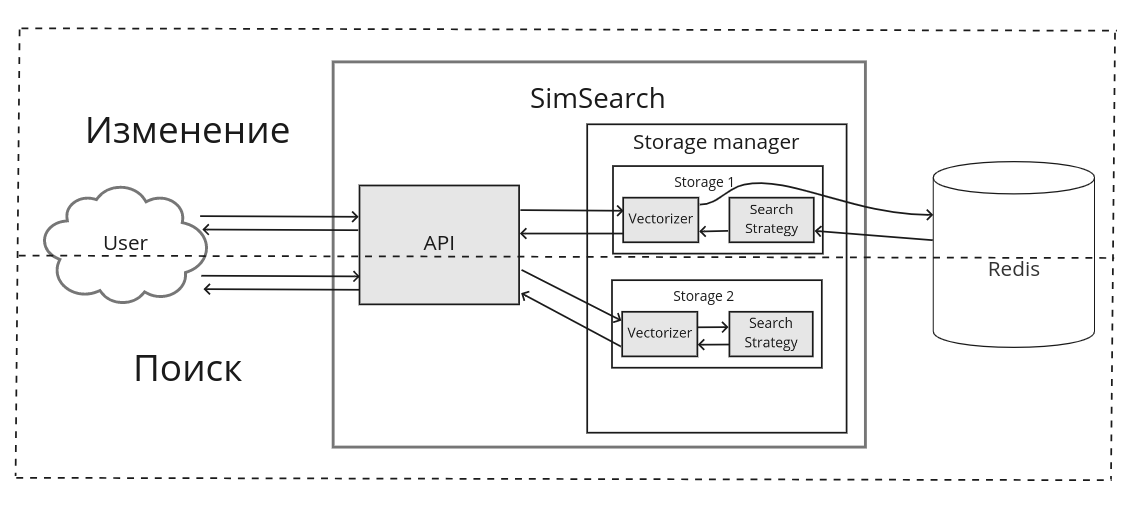
\includegraphics[width=\linewidth]{miro_4.png}
\end{center}

\end{frame}

\begin{frame}
\frametitle{SimSearch: масштабируемость, Redis}

\begin{center}
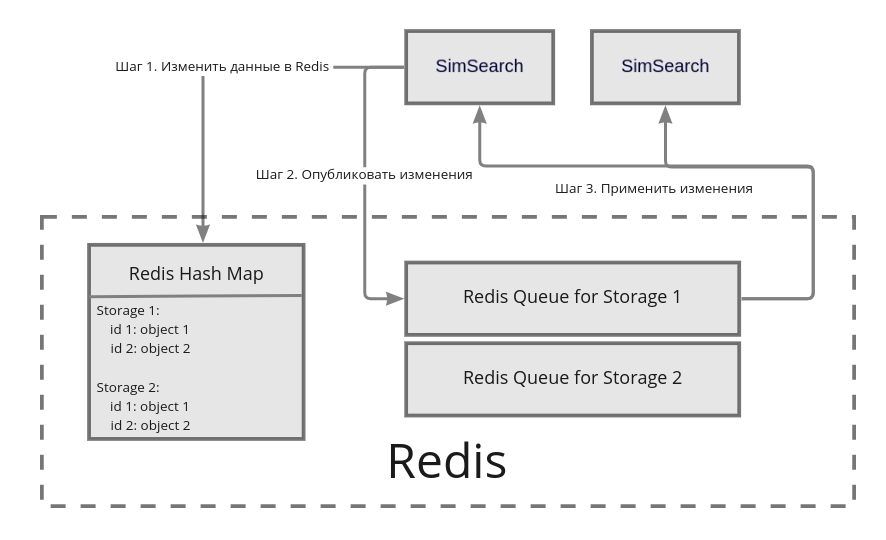
\includegraphics[width=\linewidth]{miro_1.png}
\end{center}

\end{frame}

\begin{frame}
\frametitle{SimSearch: тестирование}

\centering
\begin{tabular}{|c|c|c|c|}
\hline
    Стратегия & Размер хранилища &  t(Add), мс & t(Search), мс \\
     \hline
    linear & 1000 & 12 & 98 \\
    \hline 
    linear & 5000 & 11 & 410 \\
    \hline 
    lshkit & 1000 & 89 & 14 \\
    \hline 
    lshkit & 5000 & 280 & 25 \\
    \hline 
    faiss-hnsw & 1000 & 12 & 43.5 \\
    \hline 
    faiss-hnsw & 5000 & 14 & 44 \\
    \hline 
\end{tabular}

\hfill

\textbf{Вывод:} для статической поисковой задачи лучше использовать стратегию с lshkit, для динамической --- faiss-hnsw.

\end{frame}

\begin{frame}
\frametitle{SimSearch: что еще?}

\begin{itemize}
\item Cmake: сборка
\item Docker: контейнеризация
\item Pytest: тесты
\item CI/CD в Gitlab  
\end{itemize}

\end{frame}

\begin{frame}
\frametitle{Поиск похожих изображений}

Приложение для демонстрации возможностей SimSearch. Разработано на flask, взаимодействует с API SimSearch.

\begin{center}
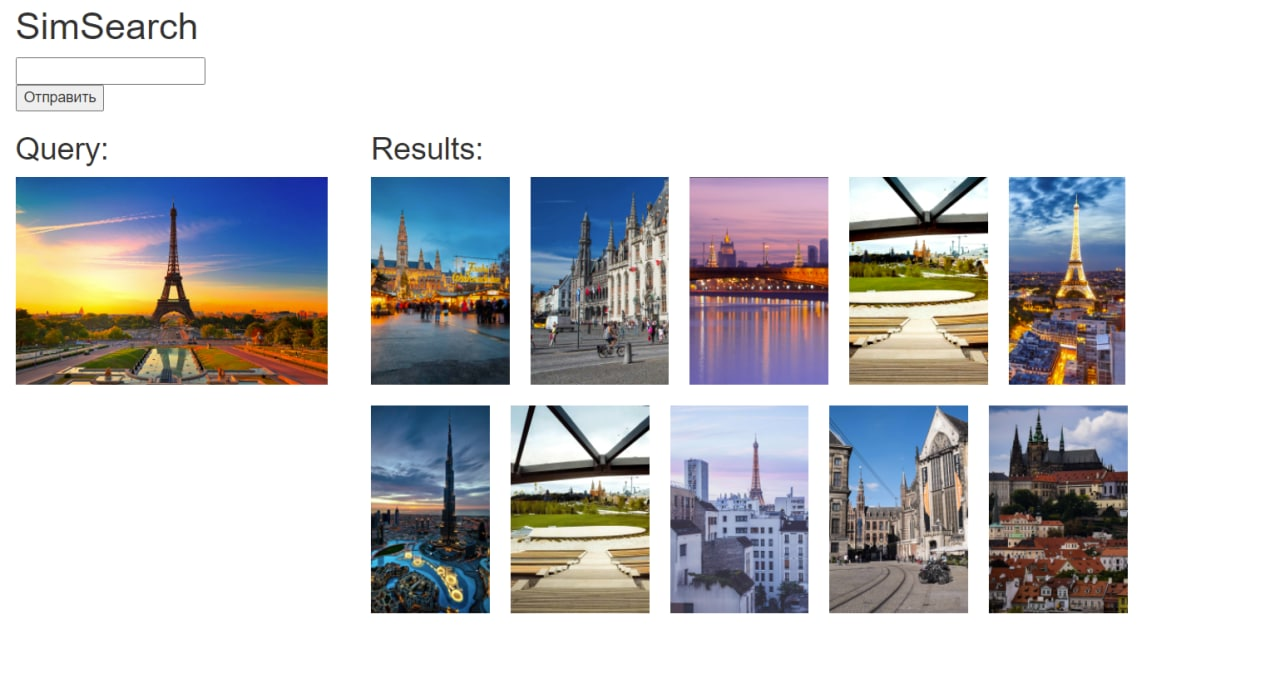
\includegraphics[width=\linewidth]{simsearch_paris.jpg}

\end{center}


\end{frame}

\begin{frame}
\frametitle{Поиск похожих изображений: еще примеры}


\begin{center}
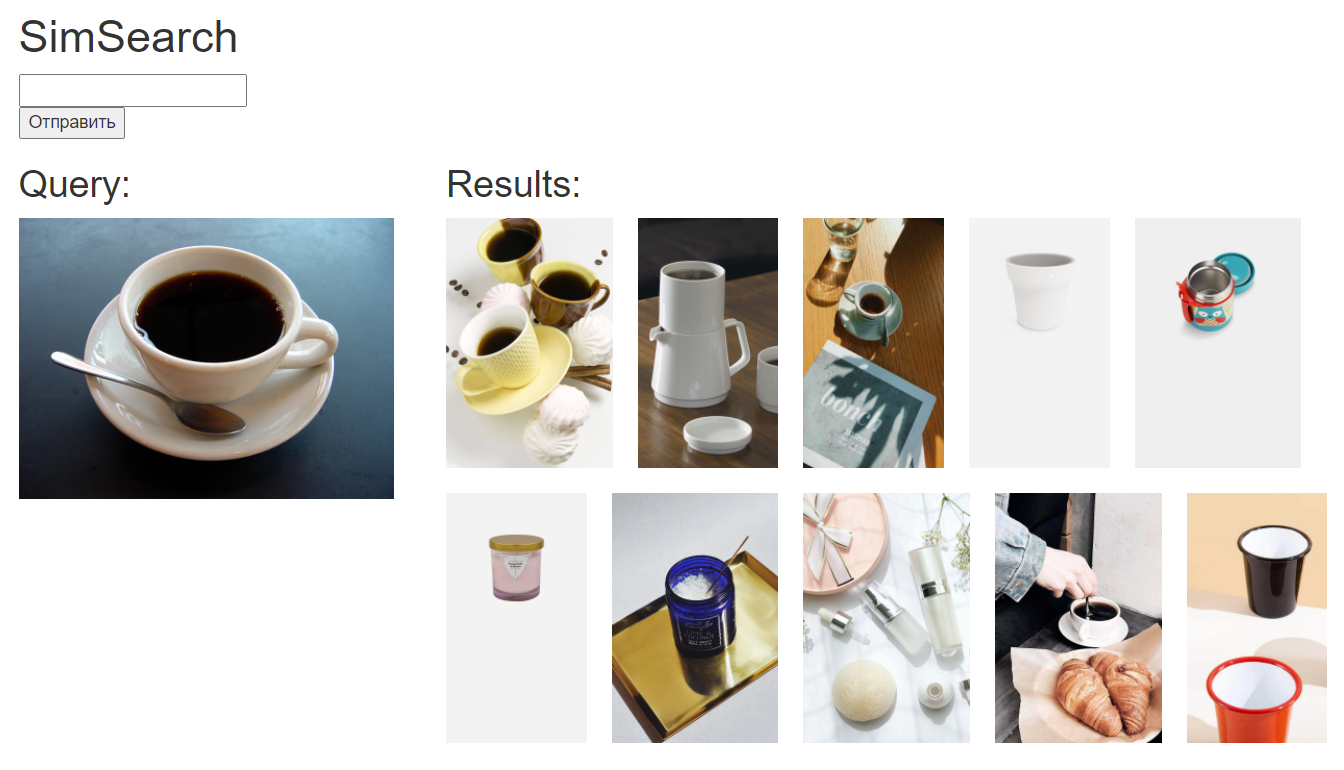
\includegraphics[width=\linewidth]{simsearch_coffee.png}
\end{center}


\end{frame}

\begin{frame}
\frametitle{Поиск похожих изображений: неудачные примеры}


\begin{center}
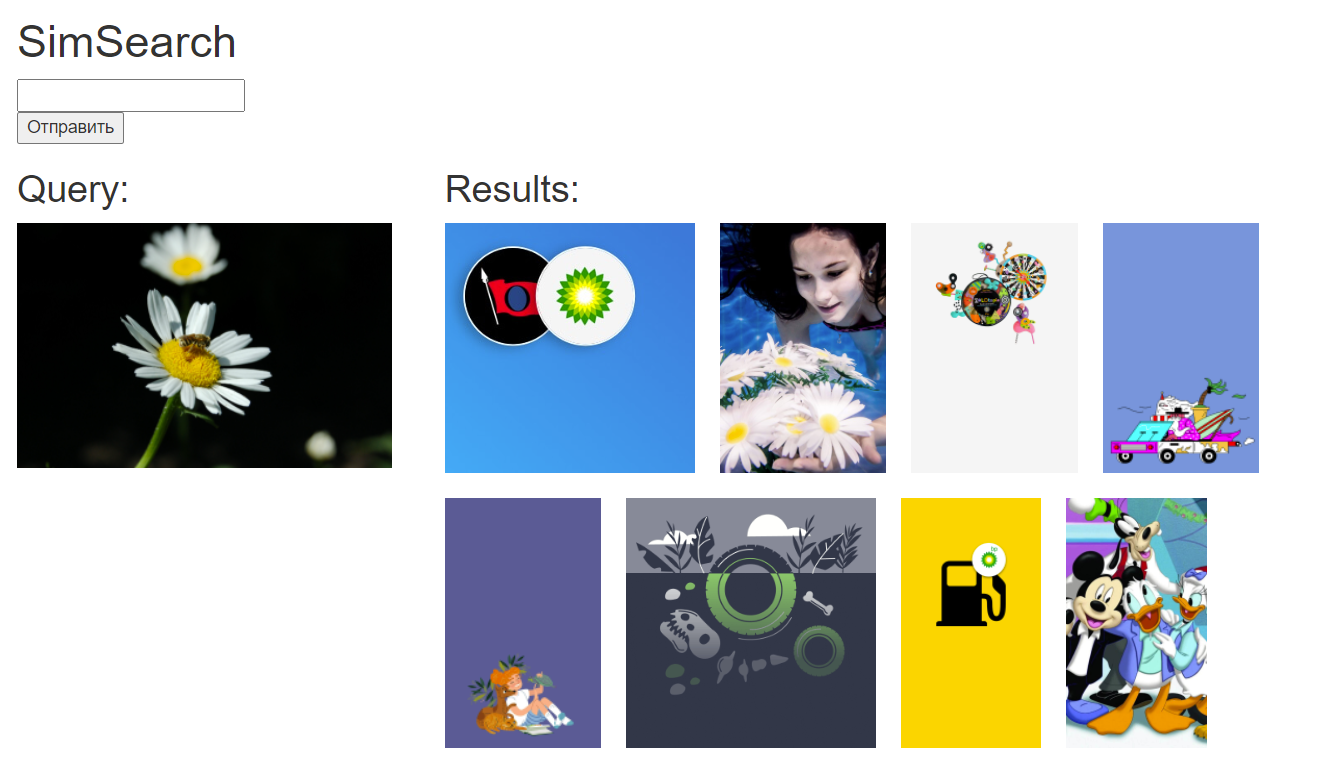
\includegraphics[width=\linewidth]{simsearch_daisy.png}
\end{center}

Узнали, что логотип топливной компании напоминает ромашку :).

\end{frame}

\begin{frame}
\frametitle{Результаты}


\begin{itemize}
\item Сформулированы требования к <<универсальному>> поисковому сервису
\item Проанализированы подходы к решению задачи ANN
\item Выбраны подходящие под требования алгоритмы
\item Найдены open-source библиотеки для реализации искомых алгоритмов
\item Разработан поисковый сервис SimSearch
\item Проведено сравнение производительности поисковых стратегий
\item Разработан поиск похожих изображений с UI на основе SimSearch
\end{itemize}

\end{frame}

\begin{frame}
\frametitle{Возможности дальнейшего развития}

\begin{itemize}
\item Продолжение исследования задачи ANN
\item Добавление новых поисковых стратегий и векторизаторов
\end{itemize}

\end{frame}

\begin{frame}
\frametitle{Сервис поиска соседних объектов}

\begin{center}
Спасибо за внимание!
\end{center}
\end{frame}


\end{document}
